%%%%%%%%%%%%%%%%%%%%%%% file template.tex %%%%%%%%%%%%%%%%%%%%%%%%%
%
% This is a general template file for the LaTeX package SVJour3
% for Springer journals.          Springer Heidelberg 2010/09/16
%
% Copy it to a new file with a new name and use it as the basis
% for your article. Delete % signs as needed.
%
% This template includes a few options for different layouts and
% content for various journals. Please consult a previous issue of
% your journal as needed.
%
%%%%%%%%%%%%%%%%%%%%%%%%%%%%%%%%%%%%%%%%%%%%%%%%%%%%%%%%%%%%%%%%%%%
%
% First comes an example EPS file -- just ignore it and
% proceed on the \documentclass line
% your LaTeX will extract the file if required

\begin{filecontents*}{example.eps}
%!PS-Adobe-3.0 EPSF-3.0
%%BoundingBox: 19 19 221 221
%%CreationDate: Mon Sep 29 1997
%%Creator: programmed by hand (JK)
%%EndComments
gsave
newpath
  20 20 moveto
  20 220 lineto
  220 220 lineto
  220 20 lineto
closepath
2 setlinewidth
gsave
  .4 setgray fill
grestore
stroke
grestore
\end{filecontents*}
%
\RequirePackage{fix-cm}
%
%\documentclass{svjour3}                     % onecolumn (standard format)
%\documentclass[smallcondensed]{svjour3}     % onecolumn (ditto)
\documentclass[smallextended]{svjour3}       % onecolumn (second format)
%\documentclass[twocolumn]{svjour3}          % twocolumn
%
\smartqed  % flush right qed marks, e.g. at end of proof
%
\usepackage{graphicx}

\usepackage{amssymb, mathtools, bm}
\usepackage{subfig}
\usepackage{color} 
\captionsetup[figure]{labelfont=bf,textfont=normal, labelsep=space}
\captionsetup[table]{labelfont=bf,textfont=normal, labelsep=space}

\DeclareMathOperator{\sgn}{\mathop{sgn}}
\DeclareMathOperator*{\argmin}{arg\,min}
\newcommand{\T}{{\mbox{\scriptsize\sffamily\upshape\mdseries T}}}
%
% \usepackage{mathptmx}      % use Times fonts if available on your TeX system
%
% insert here the call for the packages your document requires
%\usepackage{latexsym}
% etc.
%
% please place your own definitions here and don't use \def but
% \newcommand{}{}
%
% Insert the name of "your journal" with
% \journalname{myjournal}
%
\begin{document}

\title{Feature Generation for Physical Activity Classification%\thanks{Grants or other notes
%about the article that should go on the front page should be
%placed here. General acknowledgments should be placed at the end of the article.}
}

%\titlerunning{Short form of title}        % if too long for running head

\author{Roman Isachenko         \and
        Ilya Zharikov \and
        Artem Bochkarev \and
        Vadim Strijov.
}

%\authorrunning{Short form of author list} % if too long for running head

\institute{Roman Isachenko \at
				Moscow Institute of Physics and Technology, 9 Institutskiy Per., Dolgoprudny 141700, Russian Federation \\
				\email{isa-ro@yandex.ru}
				\and
				Ilya Zharikov \at
				Moscow Institute of Physics and Technology, 9 Institutskiy Per., Dolgoprudny 141700, Russian Federation \\
				\email{ilya250894@gmail.com}
				\and
				Artem Bochkarev \at
				Moscow Institute of Physics and Technology, 9 Institutskiy Per., Dolgoprudny 141700, Russian Federation \\
				\email{artem.bochkarev@phystech.edu}
				\and
				Vadim Strijov \at
				A. A. Dorodnicyn Computing Centre, Federal Research Center “Computer Science and Control” of the Russian Academy of Sciences, 40 Vavilov Str., Moscow 119333, Russian Federation \\
				\email{strijov@ccas.ru}
				\and
				This research was supported by RFBF project 16-07-01154.
				} 
	


\date{Received: date / Accepted: date}
% The correct dates will be entered by the editor


\maketitle

\begin{abstract}
	The paper investigates the human physical activity classification problem.
	Time series from accelerometer of a wearable device produce a dataset.
	Due to high dimension of the object description and low computational resources one has to state a feature generation problem.
	The authors propose to use parameters of the local approximation models as informative features. 
	The experiment is conducted on two datasets for human activity recognition using accelerometer: WISDM and USC-HAD. 
	It compares several superpositions of various generation and classification models.
	\keywords{wearable devices, accelerometer, time series, local approximation, classification}
\end{abstract}

\section{Introduction}
The paper investigates the multiclass classification problem of objects with no explicit feature representation. This problem arises in analysing biological data~\cite{motrenko2016extracting}, human behavior and social interactions~\cite{bao2004activity}. It considers the problem of human activity recognition.
The accelerometer time series~\cite{ignatov2016human,lu2016towards,wang2014human} from smart phones serve to recognize human physical activity in the internet of things~\cite{budnik2017learned,lu2016activity}.
Methods to solve this problem range from topological data analysis~\cite{umeda2017time} to convolutional neural networks~\cite{hammerla2016deep}. 
The extensive survey of methods and datasets for this problem is in~\cite{incel2013review}. 

In this work the dataset collects time series of acceleration from three axis, which is obtained from a mobile phone or another wearable device with accelerometer. 
These time series are of various sizes, not aligned and multiscaled~\cite{geurts2001pattern}.
The problem is to predict physical activity of a person. 
The list of activities includes walking, running, sitting or walking up/down stairs.
In this setup the time series are treated as complex structured objects without explicit feature description. 
This assumption allows to propose a flexible technology of accelerometer time series modelling. 
The main problem to tackle is the lack of computational resources, memory and energy in wearable devices. 
This investigation proposes an approach to generate features of time series as complex structured objects. 
The generated features bring adequate quality of classification and require moderate resources.

The problem of classifying complex structured objects is split in two distinctive procedures. 
The first extracts informative features. The second one classifies objects of these feature descriptions.
This research focuses mainly on comparison of different methods of feature generation~\cite{karasikov2016feature,ivkin2015ts}: expert-defined functions, autoregressive model and singular spectrum analysis.
The expert-defined functions~\cite{kwapisz2011activity} include the average, standard deviation, mean absolute deviation and histogram. The autoregressive model~\cite{lukashin2003adaptive} builds a parametric model for each time series and use parameters of the model as features for classification. The singular spectrum analysis~\cite{hassani2007singular} uses the eigenvalues of trajectory matrix as generated features.

The authors propose a new feature generation method. 
We approximate time series segments with cubic splines~\cite{deboor1978splines}. 
The spline approximates the 3-order piecewise curve at the given knots. The additional smoothess conditions makes the curve and its first and second derivatives continuous. The splines give a smooth curve and adequate quality of approximation.

The experiment was conducted on two accelerometer datasets: WISDM~\cite{wisdm}, USC-HAD~\cite{usc}. 
We compared the performance of stated feature extraction methods, as well as different classification algorithms. 
The latter include logistic regression, random forest and SVM.

\section{Problem Statement}
The accelerometer time series is represented as a set $\mathcal{S}$ of segments $s$ of fixed length~$T$:
\begin{equation}
s = [x_1, \dots, x_T]^{\T} \in \mathbb{R}^T.
\label{eq::time_series}
\end{equation}
One has to find a classification model $f: \mathbb{R}^T \rightarrow Y$ between segments from the set $\mathcal{S}$ and class labels from a finite set $Y$.
Denote by 
\begin{equation}
\mathcal{D} = \{(s_i, y_i)\}_{i=1}^m
\label{eq::sample}
\end{equation}
a~given sample set, where $s_i \in \mathcal{S}$ and $y_i = f(s_i)\in Y$.

The authors propose to construct the model $f$ as a superposition $f=f(\bm{g})$.
Here $\bm{g}: \mathbb{R}^T \rightarrow \mathbb{R}^n$ is a map from the space $\mathbb{R}^{T} $ to the feature space $G \subset \mathbb{R}^n$.
Given the feature map $\bm{g}$ transform the original sample set~\eqref{eq::sample} to the new sample set
\[
\mathcal{D}_G = \{(\bm{g}_i, y_i)\}_{i=1}^m,
\]
where $\bm{g}_i = \bm{g}(s_i) \in G$. 

The classification model $f=f(\bm{g}, \bm{\theta})$ has a vector of parameters $\boldsymbol{\theta}$. 
The optimal parameters~$\hat{\bm{\theta}}$ are given by the classification error function
\begin{equation}
\hat{\bm{\theta}} = \argmin_{\bm{\theta}} L(\bm{\theta}, \mathcal{D}_G, \bm{\mu}).
\label{eq::optimal_classification_params}
\end{equation}
Here the vector $\bm{\mu}$ is external parameters of a particular classification model. The examples of these parameters and error functions for different classification models are given below.

To compare classification quality with results from~\cite{karasikov2016feature,ivkin2015ts} use the accuracy score:
\begin{equation}
\mathrm{accuracy} = \frac{1}{m} \sum_{i=1}^{m} \left[f\left(\bm{g}(s_i), \hat{\bm{\theta}} \right)= y_i\right].
\label{eq::accuracy}
\end{equation}

\section{Feature Generation Functions}

The main focus of this paper is to compare different approaches for feature generation. 
In this section we provide analysis and motivation for each of the methods.

\subsection{Expert Functions}

Use the expert-given feature set as the baseline for local approximation models.
These functions are statistics $g_j$, where $g_j: \mathbb{R}^T \rightarrow \mathbb{R}$.
The description $\bm{g}(s)$ of the object $s$ is the value of these statistics on the object 
\[
\bm{g}(s) = [g_1(s), \dots, g_n(s)]^{\T}.
\]

In paper~\cite{kwapisz2011activity} the authors proposed to use the expert functions listed in table~\ref{tbl::expert_functions}.
This feature generation procedure extracts the feature description of time series $\bm{g}(s) \in \mathbb{R}^{40}$.

\begin{table}[h]
	\centering
	\caption{Expert functions}
	\begin{tabular}{|l|c|}
		\hline
		\textbf{Function description}    & \textbf{Formula} \\ \hline
		Mean                    & $\bar{x} = \frac{1}{T} \sum_{t=1}^{T} x_t$    \\ \hline
		Standard deviation      & $\sqrt{\frac{1}{T} \sum_{t=1}^{T} (x_t - \bar{x})^2}$    \\ \hline
		Mean absolute deviation & $\frac{1}{T} \sum_{t=1}^{T} |x_t - \bar{x}|$    \\ \hline
		Distribution            &  Histogram values with 10 bins    \\ \hline
	\end{tabular}
	\label{tbl::expert_functions}
\end{table}

\subsection{Autoregressive Model}
The autoregressive model~\cite{lukashin2003adaptive} of the order $n$ generates features of time series $s$ with model parameters. 
Each time series is approximated by a linear combination of its previous $n-1$ components 
\begin{equation*}
x_t = w_0 + \sum_{j=1}^{n-1} w_j x_{t-j} + \epsilon_t,
\end{equation*}
where $\epsilon_t$ is a residual. 
The optimal parameters $\hat{\bm{w}}$ of the autoregressive model are the features $\bm{g}(s)$.
These parameters minimize the squared error between the time series $s$ and its prediction

\begin{equation}
\bm{g}(s) = \hat{\bm{w}} = \argmin_{\bm{w} \in \mathbb{R}^{n}} \left( \sum_{t=n}^{T} \|x_t - \hat{x}_t\|^2\right).
\label{eq::autoregressive_description}
\end{equation}
The problem~\eqref{eq::autoregressive_description} is a linear regression problem. Hence, for each initial time series~$s$ we have to solve linear regression problem with $n$ predictors.
The example of approximation using autoregressive model is demonstrated on the Fig.~\ref{fig::ar_example}.

\begin{figure}[h]
	\centering
	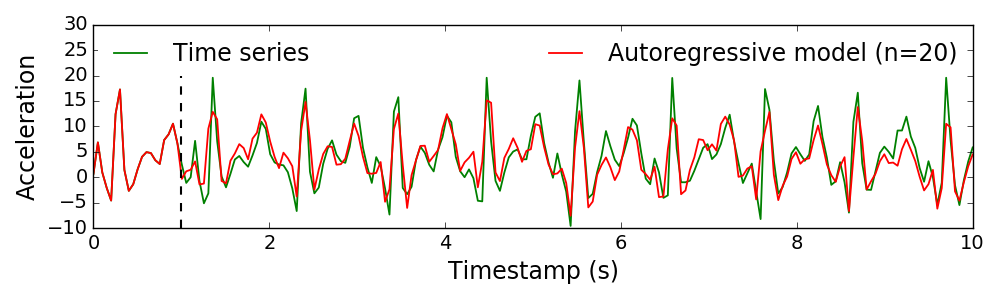
\includegraphics[width=1\linewidth]{pics/Fig1.png}
	\caption{Time series approximation using autoregressive model with order $n = 20$}
	\label{fig::ar_example}
\end{figure}

\subsection{Singular Spectrum Decomposition}
Alternative hypothesis for generation of time series is Singular Spectrum Analysis (SSA) model~\cite{hassani2007singular}. We construct trajectory matrix for each time series $s$ from the original sample $\mathcal{D}$:
\[
\mathbf{X} = 
\begin{pmatrix}
x_1 & x_2 & \dots & x_n \\
x_2 & x_3 & \dots & x_{n+1} \\
\dots & \dots & \dots & \dots \\
x_{T-n+1} & x_{T-n+2} & \dots & x_T
\end{pmatrix}.
\]
Here $n$ is the window width, which is an external structure parameter.
The singular decomposition~\cite{golub1970singular} of the matrix $\mathbf{X}^{\T} \mathbf{X}$:
\[
\mathbf{X}^{\T} \mathbf{X} = \mathbf{U} \mathbf{\Lambda} \mathbf{U}^{\T},
\]
where $\mathbf{U}$ is a unitary matrix and $\Lambda = \mathrm{diag}(\lambda_1, \dots, \lambda_n)$ whose entries $\lambda_i$ are eigenvalues of $\mathbf{X}^{\T} \mathbf{X}$. 
The spectrum of the matrix $\mathbf{X}^{\T} \mathbf{X}$ is used as feature description of the object $s$:
\[
\bm{g}(s) = \left[\lambda_1, \dots, \lambda_n\right]^{\T}.
\]
\subsection{Spline Approximation}
The proposed method approximates time series with splines~\cite{deboor1978splines}. A spline is defined by its parameters: knots and coefficients.
The set of knots $\{\xi_\ell\}_{\ell=0}^M$ are uniformly distributed over time series.
The models, which are built on each the interval $[\xi_{\ell-1}; \xi_{\ell}]$, are given by the coefficients $\{\mathbf{w}_\ell\}_{\ell=1}^{M}$.
\begin{figure}[h]
	\centering
	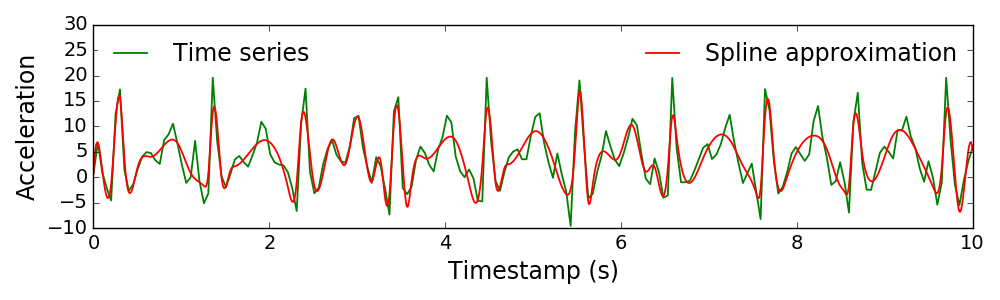
\includegraphics[width=1\linewidth]{pics/Fig2.png}
	\caption{Time series approximation using three order splines}
	\label{fig::spline_example}
\end{figure}
Optimal spline parameters are solution of a system with additional constraints of equality of derivatives up to second order on the edges of intervals. Denote each spline segment as $p_i(t)$ $i = 1, \dots, M$ and spline as a whole as $S(t)$ and write these equations:
\begin{align*}
S(t) &= \begin{cases}
p_1(t) = w_{10} +w_{11}t + w_{12}t^2 + w_{13}t^3, & t\in [\xi_0, \xi_1],\\
p_2(t) = w_{20} +w_{21}t + w_{22}t^2 + w_{23}t^3, & t\in [\xi_1, \xi_2],\\
\cdots&\cdots \\
p_{M}(t) = w_{L0} +w_{M1}t + w_{M2}t^2 + w_{M3}t^3, & t\in [\xi_{M-1}, \xi_M],					
\end{cases}
\end{align*}
For $S(t)$ to be an interpolatory cubic spline, we must also have conditions:
\begin{align*}
S(\xi_t) &= x_t, \quad t = 0, \dots, M,\\
p_i'(\xi_i) &= p_{i+1}'(\xi_i),\: p_i''(\xi_i) = p_{i+1}''(\xi_i), \quad i = 1, \dots, M-1,\\
p_i(\xi_{i-1}) &= x_{i-1},\: p_i(\xi_i) = x_i, \quad i = 1, \dots, M.
\end{align*}
The feature description of the time series could be assumed as a union of the spline parameters:
\[
\bm{g}(s) = \left[\bm{w}_1, \dots, \bm{w}_{M}\right]^{\T}.
\]

Fig.~\ref{fig::spline_example} shows the time series approximation given by splines. 
Compared to the autoregressive model, the splines method gives smoother approximation using almost the same number of parameters.

\section{Time Series Classification}
Multiclass classification uses one-vs-rest approach to train binary classifiers for each class label and then, on the prediction step, classify new object according to the most confident classifier. Three classification models are used: logistic regression, SVM and random forest.

\subsection{Regularized Logistic Regression}
The optimal model parameters~\eqref{eq::optimal_classification_params} is determined by minimising the error function

\begin{equation*}
L(\bm{\theta}, \mathcal{D}_G, \mu) = \sum_{i=1}^{m} \log\bigl(1 + \exp(-y_i [\bm{w}^{\T} \bm{g}_i + b])\bigl) + \frac{\mu}{2} \|\bm{w}\|^2, \:\:\mbox{where}\:\: \bm{\theta}  = \begin{bmatrix}
\bm{w} \\ b
\end{bmatrix}.
\end{equation*}
Thus, the optimal parameters $\hat{\bm{w}}, \hat{b}$ is given by~\eqref{eq::optimal_classification_params}.

The classification rule $f(\bm{g}, \bm{\theta})$ is given by sign of the linear combination for the object description $\bm{g}$ and parameters $\hat{\bm{\theta}}$
\begin{equation*}
\hat{y} = f(\bm{g}, \hat{\bm{\theta}}) = \sgn(\bm{g}^{\T} \hat{\bm{w}} + \hat{b}).
\end{equation*}

\subsection{SVM}
The optimization problem is
\begin{align*}
\hat{\bm{\theta}}  = \begin{pmatrix}
\hat{\bm{w}} \\ \hat{b} \\ \hat{\bm{\xi}}
\end{pmatrix}= \argmin_{\bm{w}, b, \bm{\xi}}  \frac{1}{2} \|\bm{w}\|^2 + \mu \sum_{i=1}^{m} \xi_i,\:\:
\mbox{s.t.} \:\: &y_i \left(\bm{w}^{\T} \bm{g}_i + b\right) \geq 1 - \xi_i,\\
&\xi_i \geq 0, \quad 1 \leq i \leq m.
\end{align*}
The objective function corresponds to the classification error function $L(\bm{\theta}, \mathcal{D}_G, \mu)$.
The prediction for new object is $
\hat{y} = \sgn (\bm{g}^{\T} \hat{\bm{w}} + \hat{b})$.

\subsection{Random Forest}
The random forest exploits the idea of bagging. This is an approach of building many random unstable classifiers and aggregating their predictions. This method works especially well if as base models we select models with low bias and high variance (due to aggregating variance is reduced). In case of random forest decision trees take the role of base models, also not only objects are used for bagging, but also features. In this case we make the prediction for each new object as the mean of the predictions of a single tree:

\begin{equation*}
\hat{y} = \frac{1}{B} \sum_{i=1}^{B} \text{pred}(\bm{g}_i),
\end{equation*}
where $B$ is an amount of trees used for bagging.

\section{Experiment}
In this paper we considered two different smart phone based datasets: WISDM~\cite{wisdm} and USC-HAD~\cite{usc}. 
The smart phone accelerometer measures acceleration along three axis with frequencies equal to 20 and 100 Hz. 
The WISDM dataset consists of 4321 time series. Each time series belongs to one of the six activities: Standing, Walking, Upstairs, Sitting, Jogging, Downstairs. The USC-HAD dataset contains 13620 time series with one of the twelve class labels: Standing, Elevator-up,Walking-forward, Sitting, Walking-downstairs, Sleeping, Elevator-down, Walking-upstairs, Jumping, Walking-right, Walking-left, Running.
Table~\ref{tbl::activities_distributions} shows the distributions of time series activities for each datasets. 
The length $T$ of each time series equals 200. 
Fig.~\ref{fig::ts_example} plots the example of the time series for one activity of the specific person is given.

\begin{table}[!ht]
	\centering
	\caption{Distributions of the classes}
	\subfloat[WISDM]{
		\begin{tabular}{|r|l|rr|}
			\hline
			&\textbf{Activity}   & \multicolumn{2}{l|}{\textbf{\# objects}} \\
			\hline
			1&Standing            &229      &5.30  \% \\
			2&Walking             &1917     &44.36 \% \\
			3&Upstairs            &466      &10.78 \% \\
			4&Sitting             &277      &6.41  \% \\
			5&Jogging             &1075     &24.88 \% \\
			6&Downstairs          &357      &8.26  \% \\
			\hline
			&Total & \multicolumn{2}{l|}{4321}  \\
			\hline
	\end{tabular}}
	\hspace{0.5cm}
	\subfloat[USC-HAD]{
		\begin{tabular}{|r|l|rr|}
			\hline
			&\textbf{Activity} & \multicolumn{2}{l|}{\textbf{\# objects}} \\ \hline
			1&Standing            &1167     &8.57  \% \\
			2&Elevator-up         &764      &5.61  \% \\
			3&Walking-forward     &1874     &13.76 \% \\
			4&Sitting             &1294     &9.50  \% \\
			5&Walking-downstairs  &951      &6.98  \% \\
			6&Sleeping            &1860     &13.66 \% \\
			7&Elevator-down       &763      &5.60  \% \\
			8&Walking-upstairs    &1018     &7.47  \% \\
			9&Jumping             &495      &3.63  \% \\
			10&Walking-right       &1305     &9.58  \% \\
			11&Walking-left        &1280     &9.40  \% \\
			12&Running             &849      &6.23  \% \\
			\hline 
			&Total              & \multicolumn{2}{l|}{13620}\\ 
			\hline
	\end{tabular}}
	\label{tbl::activities_distributions}
\end{table}

\begin{figure}[!h]
	\centering
	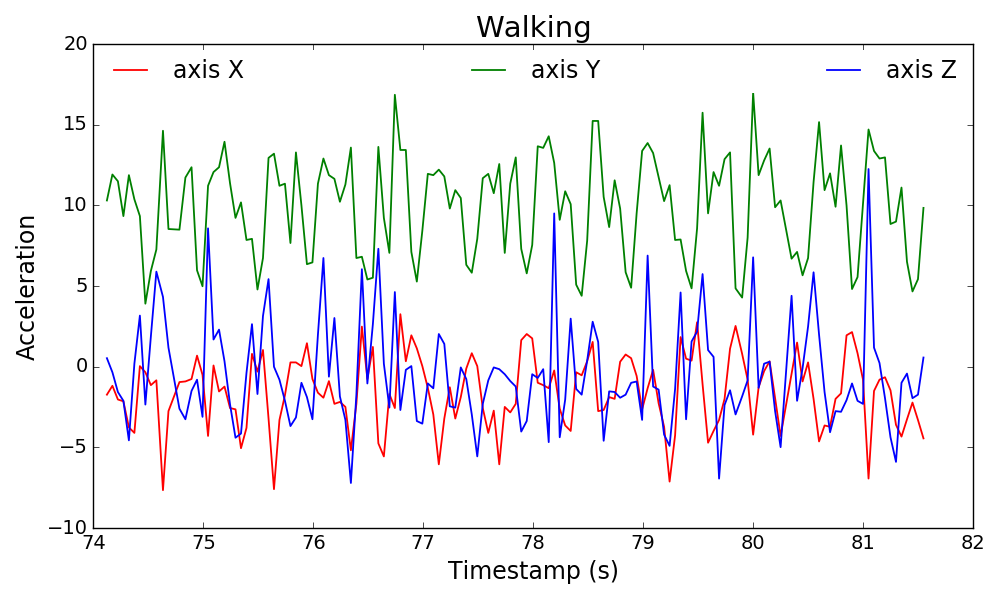
\includegraphics[width=1\linewidth]{pics/Fig3.png}
	\caption{Time series example}
	\label{fig::ts_example}
\end{figure}

\begin{figure}[!h]
	\centering
	\subfloat{
		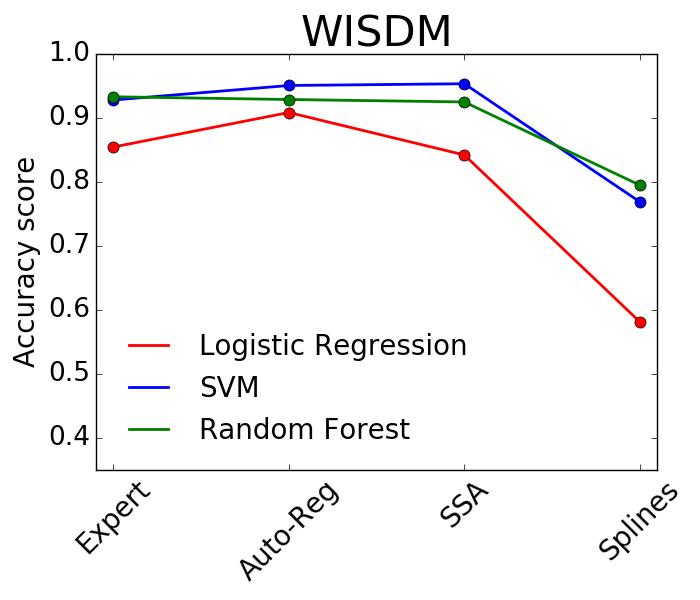
\includegraphics[width=0.49\linewidth]{pics/Fig4a.png}}
	\subfloat{
		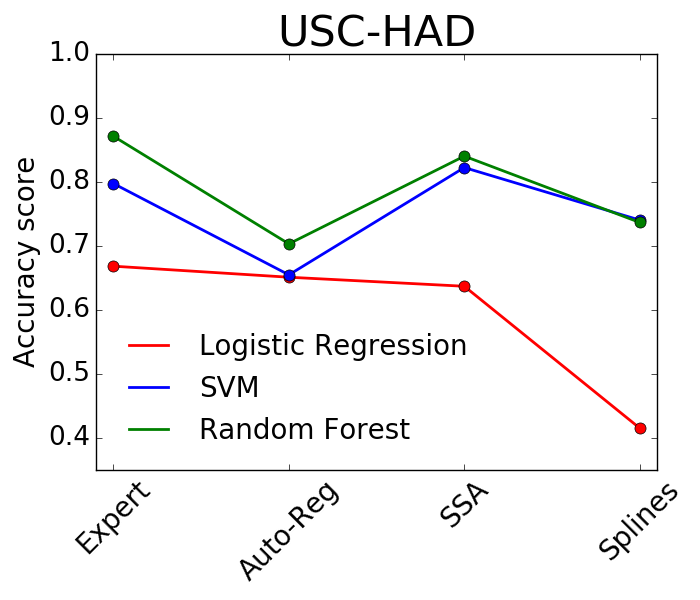
\includegraphics[width=0.49\linewidth]{pics/Fig4b.png}}
	\caption{Multiclass accuracy score}
	\label{fig::accuracy_results}
\end{figure}

For each dataset apply feature generation procedures: expert functions, autoregressive model, SSA and splines. 
Three classification models for each generated feature description: logistic regression, support vector machine and random forest. 
The structure parameters: the length $n$ for autoregressive model, the window width $n$ for SSA and the number of splines knots $M$ were tuned using K-fold cross validation, minimizing
\begin{align}\label{cv}
CV(K) = \frac{1}{K}\sum_{k=1}^{K} L(f_k, \mathcal{D}\setminus \mathcal{C}_k),
\end{align}
where $C_k$ is a $\frac{K-1}{K}$ fraction of data, used for training model $f_k$.
The hyperparameters $\bm{\mu}$ for classification models were also tuned using the same cross validation procedure. 


The first approach for feature generation is expert functions. The main drawback of this approach is a restriction by the choice of the expert functions and these functions might be impossible to derive for some types of data.

The autoregressive model was tuned to find the optimal length $n$. Cross validation procedure gives optimal value $n=20$ for both dataset. 

The singular spectrum analysis was tuned in the same way to find the optimal window width $n$. Similar to autoregressive model, cross validation procedure gives the same value $n=20$.

\begin{figure}[!h]
	\centering
	\subfloat[WISDM dataset]{
		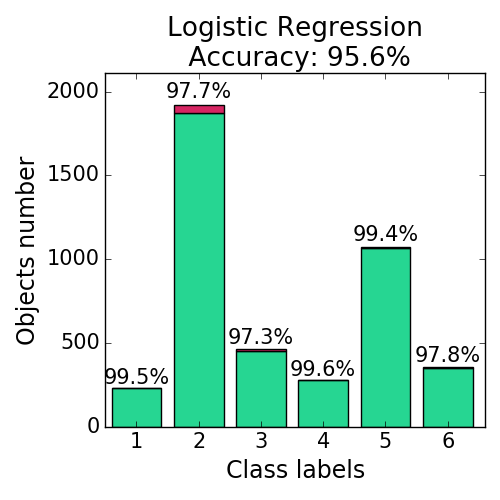
\includegraphics[width=0.33\linewidth]{pics/Fig5a.png}}
	\subfloat[USC-HAD dataset]{
		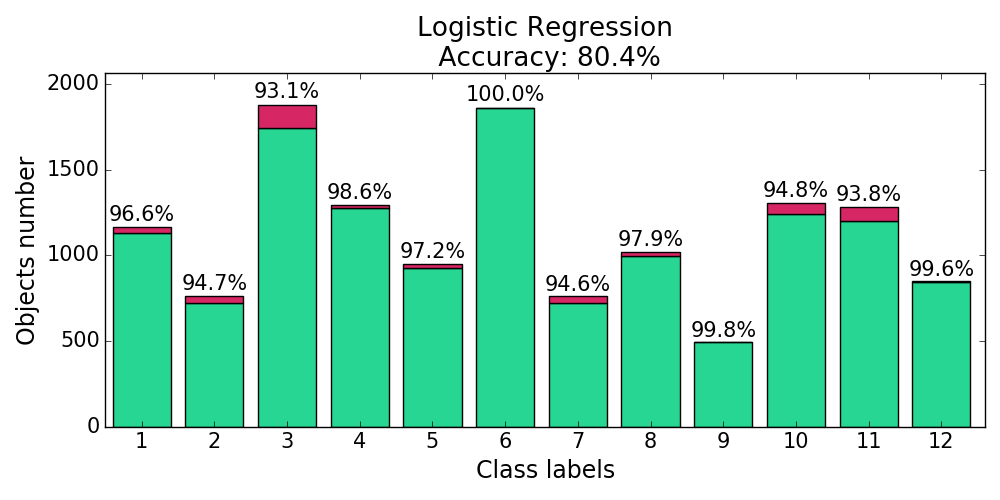
\includegraphics[width=0.66\linewidth]{pics/Fig5b.png}}\\
	\subfloat[WISDM dataset]{
		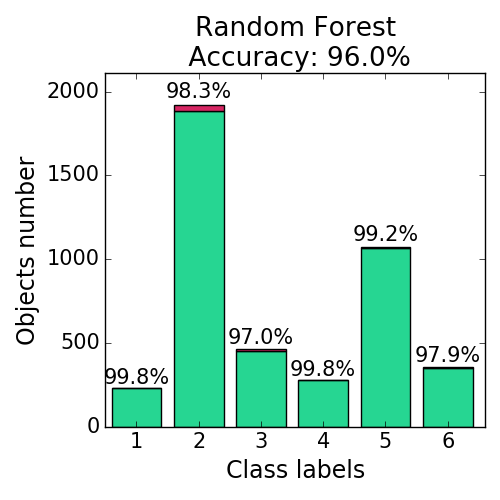
\includegraphics[width=0.33\linewidth]{pics/Fig5c.png}}
	\subfloat[USC-HAD dataset]{
		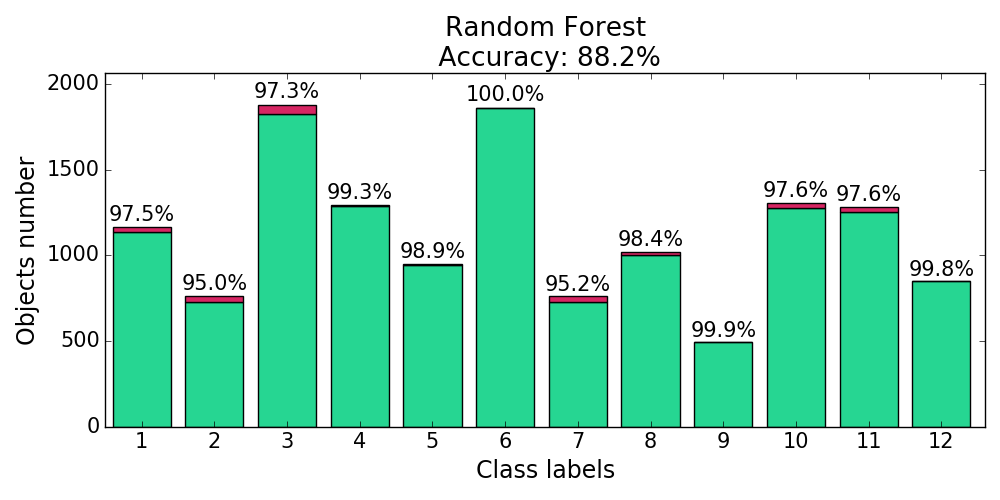
\includegraphics[width=0.66\linewidth]{pics/Fig5d.png}}\\
	\subfloat[WISDM dataset]{
		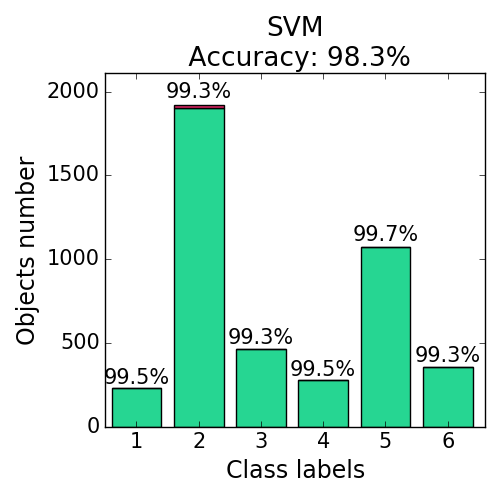
\includegraphics[width=0.33\linewidth]{pics/Fig5e.png}}
	\subfloat[USC-HAD dataset]{
		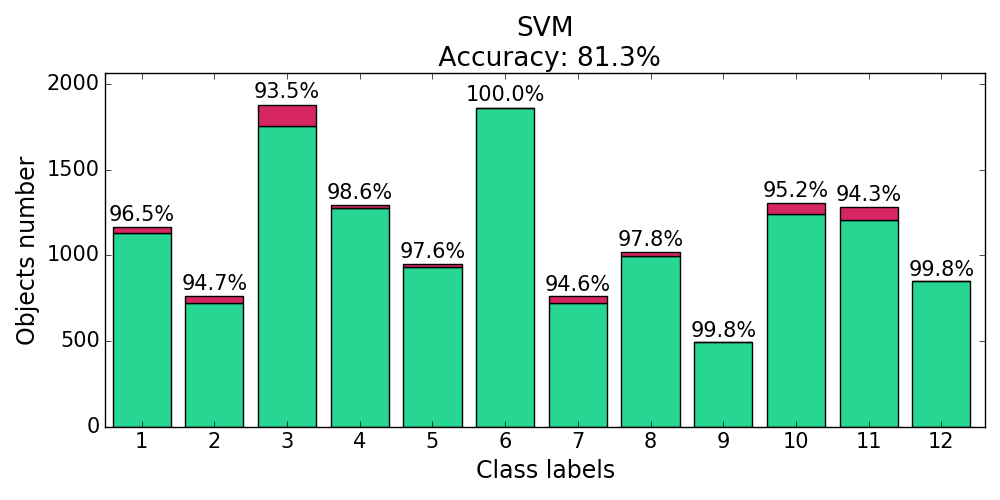
\includegraphics[width=0.66\linewidth]{pics/Fig5f.png}}\\
	\caption{Accuracy scores of classification of each class using all features}
	\label{fig::feature_union_results}
\end{figure}

Fit cubic splines~\cite{deboor1978splines} for time series using $scipy$ python library~\cite{scipy}. 
The knots $\{\xi_{\ell}\}_{\ell = 1}^M$ for splines were distributed uniformly. 
Value of~$M$ was chosen with cross validation. 

The feature extraction methods gives the following number of features for both datasets: expert features: 40; autoregressive model: 60; singular spectrum analysis: 60; splines: 33.

\begin{table}[!h]
	\centering
	\caption{Binary accuracy scores for WISDM using different feature generation methods: EX~--- Expert, AR~--- Auto-Reg, SSA,  SPL~--- Splines}
	\tiny
	\begin{tabular}{|r|rrrr|rrrr|rrrr|}
		\hline
		& \multicolumn{4}{c|}{\textbf{Logistic Regression}} & \multicolumn{4}{c|}{\textbf{Random Forest}} & \multicolumn{4}{c|}{\textbf{SVM}}          \\ \cline{2-13} 
		& EX   & AR   & SSA   & SPL  & EX  & AR & SSA & SPL & EX & AR & SSA & SPL \\ \hline
		All& 0.85 & 0.91 & 0.84 & 0.58 & 0.93 & 0.93 & 0.92 & 0.79 & 0.93 & 0.95 & 0.95 & 0.77 \\
		Standing& 0.99 & 0.98 & 1.00 & 0.95 & 1.00 & 0.99 & 1.00 & 0.99 & 0.99 & 0.98 & 1.00 & 0.96 \\
		Walking& 0.91 & 0.96 & 0.86 & 0.61 & 0.96 & 0.97 & 0.95 & 0.86 & 0.96 & 0.98 & 0.98 & 0.84 \\
		Upstairs& 0.91 & 0.95 & 0.91 & 0.89 & 0.96 & 0.96 & 0.96 & 0.90 & 0.96 & 0.98 & 0.97 & 0.89 \\
		Sitting& 0.99 & 0.98 & 1.00 & 0.99 & 1.00 & 0.99 & 1.00 & 1.00 & 0.99 & 0.98 & 1.00 & 1.00 \\
		Jogging& 0.98 & 0.99 & 0.99 & 0.80 & 0.99 & 0.99 & 0.99 & 0.92 & 0.99 & 0.99 & 0.99 & 0.93 \\
		Downstairs& 0.93 & 0.96 & 0.94 & 0.92 & 0.96 & 0.97 & 0.96 & 0.92 & 0.96 & 0.98 & 0.97 & 0.92 \\ \hline
	\end{tabular}
	\label{tbl::wisdm_methods_results}
\end{table}

\begin{table}[!h]
	\centering
	\tiny
	\caption{Binary accuracy scores for USC-HAD using different feature generation methods: EX~--- Expert, AR~--- Auto-Reg, SSA, SPL~--- Splines}
	\label{my-label}
	\begin{tabular}{|r|rrrr|rrrr|rrrr|}
		\hline
		& \multicolumn{4}{c|}{\textbf{Logistic Regression}} & \multicolumn{4}{c|}{\textbf{Random Forest}} & \multicolumn{4}{c|}{\textbf{SVM}}          \\ \cline{2-13} 
		& EX   & AR   & SSA   & SPL  & EX  & AR & SSA & SPL & EX & AR & SSA & SPL \\ \hline
		All& 0.67 & 0.65 & 0.64 & 0.41 & 0.87 & 0.70 & 0.84 & 0.74 & 0.80 & 0.65 & 0.82 & 0.74 \\
		Standing& 0.94 & 0.94 & 0.92 & 0.89 & 0.98 & 0.94 & 0.97 & 0.98 & 0.95 & 0.94 & 0.97 & 0.96 \\
		Elevator-up& 0.94 & 0.94 & 0.93 & 0.92 & 0.95 & 0.95 & 0.95 & 0.95 & 0.93 & 0.94 & 0.94 & 0.93 \\
		Walking-forward& 0.87 & 0.87 & 0.89 & 0.70 & 0.97 & 0.89 & 0.96 & 0.88 & 0.95 & 0.87 & 0.97 & 0.91 \\
		Sitting& 0.98 & 0.95 & 0.94 & 0.96 & 0.99 & 0.96 & 0.98 & 0.99 & 0.98 & 0.96 & 0.99 & 0.99 \\
		Walking-downstairs& 0.95 & 0.93 & 0.93 & 0.90 & 0.99 & 0.96 & 0.98 & 0.95 & 0.98 & 0.93 & 0.98 & 0.96 \\
		Sleeping& 1.00 & 0.98 & 0.99 & 1.00 & 1.00 & 0.98 & 1.00 & 1.00 & 1.00 & 0.98 & 1.00 & 1.00 \\
		Elevator-down& 0.94 & 0.94 & 0.94 & 0.91 & 0.95 & 0.95 & 0.95 & 0.95 & 0.93 & 0.94 & 0.94 & 0.93 \\
		Walking-upstairs& 0.94 & 0.95 & 0.93 & 0.92 & 0.98 & 0.95 & 0.98 & 0.96 & 0.98 & 0.95 & 0.98 & 0.96 \\
		Jumping& 0.99 & 0.99 & 1.00 & 0.97 & 1.00 & 0.99 & 1.00 & 0.99 & 1.00 & 0.99 & 0.97 & 0.99 \\
		Walking-right& 0.91 & 0.90 & 0.91 & 0.86 & 0.97 & 0.92 & 0.96 & 0.92 & 0.96 & 0.90 & 0.97 & 0.93 \\
		Walking-left& 0.89 & 0.91 & 0.90 & 0.88 & 0.97 & 0.93 & 0.97 & 0.93 & 0.95 & 0.91 & 0.97 & 0.93 \\
		Running& 0.99 & 0.99 & 0.99 & 0.92 & 1.00 & 0.99 & 1.00 & 0.97 & 1.00 & 1.00 & 0.95 & 0.98\\ \hline
	\end{tabular}
	\label{tbl::uschad_methods_results}
\end{table}


Fig.~\ref{fig::accuracy_results} presents the accuracy scores~\eqref{eq::accuracy} of the experiments for the both datasets. For WISDM dataset the worst result was obtained with spline approximation. 
The results for expert functions, autoregressive model and SSA is roughly identical. For USC-HAD dataset the results highly depend on the classification model. 
For both datasets logistic regression shows the worst quality, while the accuracy for support vector machine and random forest is almost the same. The spline approximation gives competitive result for USC-HAD dataset.

Table~\ref{tbl::wisdm_methods_results} and table~\ref{tbl::uschad_methods_results} presents all results with classification accuracy scores~\eqref{eq::accuracy} for each class. The first row of these tables introduces the multiclass accuracy score for each classification model and each feature extraction procedure. Next rows are related to binary accuracy scores for each class. For WISDM dataset the best scores have the least active classes such as Standing and Sitting. For USC-HAD dataset all classes have the similar accuracy scores.

We also carried out the experiment for union of all 193 generated features. Fig.~\ref{fig::feature_union_results} demonstrates the results. Table~\ref{tbl::activities_distributions} shows class labels, that are represented on the corresponding histograms. As expected, the accuracy scores for feature union are higher in all cases. All binary accuracy scores for WISDM dataset is higher than $97 \%$ for each classification model. These numbers for USC-HAD dataset is higher than $93 \%$.

\section{Conclusion}

The paper investigates the problem of complex structured objects classification.
The experiment compares various approaches of feature extraction, particularly the expert functions and local approximation models on data from smart phone accelerometer.
The logistic regression, SVM and random forest are used for classification. 
The results show that obtained features recovers the class label with the high quality. 
The proposed spline method gives smooth approximation of time series. 
The number of splines parameters was less than for the other methods. 
The classification quality for splines are competitive with existing stated methods for both considered datasets.  
Stacking of all extracted features gives better performance.

\bibliographystyle{splncs03}

\begin{thebibliography}{10}
	\providecommand{\url}[1]{\texttt{#1}}
	\providecommand{\urlprefix}{URL }
	
	\bibitem{bao2004activity}
	Bao, L., Intille, S.S.: Activity recognition from user-annotated acceleration
	data. In: International Conference on Pervasive Computing. pp. 1--17.
	Springer (2004)
	
	\bibitem{budnik2017learned}
	Budnik, M., Gutierrez-Gomez, E.L., Safadi, B., Pellerin, D., Qu{\'e}not, G.:
	Learned features versus engineered features for multimedia indexing.
	Multimedia Tools and Applications  76(9),  11941--11958 (2017)
	
	\bibitem{deboor1978splines}
	De~Boor, C.: A practical guide to splines, vol.~27. Springer-Verlag (1978)
	
	\bibitem{geurts2001pattern}
	Geurts, P.: Pattern extraction for time series classification. In: European
	Conference on Principles of Data Mining and Knowledge Discovery. pp.
	115--127. Springer (2001)
	
	\bibitem{golub1970singular}
	Golub, G.H., Reinsch, C.: Singular value decomposition and least squares
	solutions. Numerische mathematik  14(5),  403--420 (1970)
	
	\bibitem{hammerla2016deep}
	Hammerla, N.Y., Halloran, S., Ploetz, T.: Deep, convolutional, and recurrent
	models for human activity recognition using wearables. arXiv preprint
	arXiv:1604.08880  (2016)
	
	\bibitem{hassani2007singular}
	Hassani, H.: Singular spectrum analysis: methodology and comparison. Journal of
	Data Science  5(2),  239--257 (2007)
	
	\bibitem{ignatov2016human}
	Ignatov, A.D., Strijov, V.V.: Human activity recognition using quasiperiodic
	time series collected from a single tri-axial accelerometer. Multimedia tools
	and applications  75(12),  7257--7270 (2016)
	
	\bibitem{incel2013review}
	Incel, O.D., Kose, M., Ersoy, C.: A review and taxonomy of activity recognition
	on mobile phones. BioNanoScience  3(2),  145--171 (2013)
	
	\bibitem{scipy}
	Jones, E., Oliphant, T., Peterson, P.: {SciPy}: Open source scientific tools
	for {Python} (2001), \url{http://www.scipy.org/}. Accessed 1 September 2017
	
	\bibitem{karasikov2016feature}
	Karasikov, M., Strijov, V.: Feature-based time-series classification.
	Intelligence  24(1),  164--181 (2016)
	
	\bibitem{ivkin2015ts}
	Kuznetsov, M., Ivkin, N.: Time series classification algorithm using combined
	feature description. Machine Learning and Data Analysis  1(11),  1471--1483
	(2015)
	
	\bibitem{kwapisz2011activity}
	Kwapisz, J.R., Weiss, G.M., Moore, S.A.: Activity recognition using cell phone
	accelerometers. ACM SigKDD Explorations Newsletter  12(2),  74--82 (2011)
	
	\bibitem{lu2016activity}
	Lu, L., Qing-ling, C., Yi-Ju, Z.: Activity recognition in smart homes.
	Multimedia Tools and Applications pp. 1--18 (2016)
	
	\bibitem{lu2016towards}
	Lu, Y., Wei, Y., Liu, L., Zhong, J., Sun, L., Liu, Y.: Towards unsupervised
	physical activity recognition using smartphone accelerometers. Multimedia
	Tools and Applications  76(8)
	
	\bibitem{lukashin2003adaptive}
	Lukashin, Y.P.: Adaptive methods of short-term forecasting of time series. M.:
	Finance and statistics  (2003)
	
	\bibitem{motrenko2016extracting}
	Motrenko, A., Strijov, V.: Extracting fundamental periods to segment biomedical
	signals. IEEE journal of biomedical and health informatics  20(6),
	1466--1476 (2016)
	
	\bibitem{umeda2017time}
	Umeda, Y.: Time series classification via topological data analysis.
	Transactions of the Japanese Society for Artificial Intelligence  32(3),
	D--G72\_1 (2017)
	
	\bibitem{usc}
	The usc human activity dataset.
	\url{http://www-scf.usc.edu/~mizhang/datasets.html}. Accessed 1 September 2017
	
	\bibitem{wang2014human}
	Wang, W., Liu, H., Yu, L., Sun, F.: Human activity recognition using smart
	phone embedded sensors: A linear dynamical systems method. In: Neural
	Networks (IJCNN), 2014 International Joint Conference on. pp. 1185--1190.
	IEEE (2014)
	
	\bibitem{wisdm}
	The wisdm dataset. \url{http://www.cis.fordham.edu/wisdm/dataset.php}. Accessed 1 September 2017
	
\end{thebibliography}

%Author, Article title, Journal, Volume, page numbers (year)

\end{document}
% end of file template.tex

